\documentclass[11pt,a4paper]{article}
\usepackage[margin=2.5cm]{geometry}
\usepackage{amsmath,amssymb,bm}
\usepackage{graphicx,booktabs,caption,subcaption}
\usepackage{xcolor}
\usepackage[colorlinks=true,linkcolor=blue!50!black,citecolor=blue!50!black,urlcolor=blue!50!black]{hyperref}
\usepackage{enumitem}
\usepackage{microtype}
\graphicspath{{../figures/}}
\newcommand{\dd}{\mathrm{d}}
\newcommand{\Dstar}{\Delta^{\!*}}
\newcommand{\pn}{\psi_n}
\newcommand{\bB}{\bm{B}}
\newcommand{\bJ}{\bm{J}}
\newcommand{\ephi}{\hat{\bm{\varphi}}}
\newcommand{\er}{\hat{\bm{r}}}
\newcommand{\ez}{\hat{\bm{z}}}
\newcommand{\rhoS}{\rho}

\title{\textbf{A finite-difference Grad--Shafranov solver\\ on a boundary-fitted non-homogeneous mesh:\\ Solov'ev benchmark and nonlinear Picard equilibria}}
\author{Hausel-Vargha Emil}
\date{Work carried out: February--May, 2026\\ Write-up: November, 2026}

\begin{document}
\maketitle

\begin{abstract}
We built a fixed-boundary Grad--Shafranov (GS) solver written in Python. The solver follows the finite-difference scheme on a boundary-fitted non-homogeneous mesh of L\'opez, Orozco and Dougar-Zhabon~\cite{lopez2019}, which they validated only for the linear Solov'ev case, and extends it to the general nonlinear case with arbitrary $p'(\psi)$ and $FF'(\psi)$ through Picard iteration~\cite{jardin2010}. We describe the mesh construction, the discretisation, the sparse linear algebra and the iteration; we benchmark the linear solve against the analytic Solov'ev equilibrium (observed order of convergence $\approx 1.9$, maximum error $7\times10^{-6}$ on a $233\times233$ grid); we validate the nonlinear code path; we show nonlinear equilibria for several profiles and boundary shapes; and we study the spectrum of the Picard map, whose spectral radius predicts the observed number of iterations well.
\end{abstract}
\clearpage

\tableofcontents

\clearpage
%=====================================================================
\section{Context}\label{sec:context}
%=====================================================================

\subsection{What is the Grad--Shafranov equation?}
In a tokamak, the plasma is confined by a magnetic field that is, to a good approximation, symmetric under rotation about the machine axis. Writing $(r,\varphi,z)$ for cylindrical coordinates and imposing $\partial_\varphi\equiv 0$ on all scalar fields, ideal MHD in static equilibrium reduces to
\begin{equation}
\bJ\times\bB=\nabla p,\qquad \mu_0\bJ=\nabla\times\bB,\qquad \nabla\cdot\bB=0 .
\end{equation}
The divergence-free field is written through a poloidal flux function $\psi=rA_\varphi$ and a toroidal-field function $f=rB_\varphi$ as
\begin{equation}
\bB=\frac1r\nabla\psi\times\ephi+\frac{f}{r}\,\ephi .
\end{equation}
Force balance forces $p=p(\psi)$ and $f=f(\psi)$, and the remaining component of $\bJ\times\bB=\nabla p$ is the Grad--Shafranov equation
\begin{equation}
\boxed{\;\Dstar\psi=-\mu_0 r^2\frac{\dd p}{\dd\psi}-f\frac{\dd f}{\dd\psi}\;},\qquad
\Dstar\psi:=\frac{\partial^2\psi}{\partial r^2}-\frac1r\frac{\partial\psi}{\partial r}+\frac{\partial^2\psi}{\partial z^2}.
\label{eq:GS}
\end{equation}
It is a two-dimensional, elliptic, and (in general) \emph{nonlinear} PDE for $\psi(r,z)$: it looks like a Poisson problem, but the source depends on the unknown through the two free functions $p(\psi)$ and $FF'(\psi)=\tfrac12 \dd (f^2)/\dd\psi$. A full derivation is given in Appendix~\ref{app:derivation}.

\subsection{How should we interpret this equation?}
\begin{itemize}[nosep]
\item \textbf{Shape of the confinement region.} Level sets of $\psi$ are the magnetic flux surfaces. These are toroidal surfaces on which field lines lie and, to leading order, along which heat and particles flow quickly. The equilibrium describes where the plasma sits, its elongation and triangularity, and the Shafranov shift of the magnetic axis. 
\item \textbf{Operation, design.} Real-time reconstruction codes solve GS from magnetic measurements to control the plasma shape; design studies use it to explore shapes and profile scenarios before building anything.
\item \textbf{Physics.} The GS solution gives the current density $\bJ$ and the magnetic field $\bB$, which are used to compute the safety factor $q(\psi)$, the magnetic shear, the Shafranov shift, and other quantities that enter stability and transport calculations.
\end{itemize}

\subsection{Fixed versus free boundary, direct versus inverse}
\paragraph{Fixed boundary.} The last closed flux surface is prescribed (here by a parametric D-shape, or by a Solov'ev contour), $\psi=\psi_b$ is imposed on it, and \eqref{eq:GS} is solved only inside. The exterior is irrelevant. Choosing the profiles $p(\psi)$, $FF'(\psi)$ and the shape then gives $\psi$, and in a real device the pressure profile and toroidal field are controllable to a good extent, so scanning shape and profile weights is an inexpensive way to build intuition. This is the problem treated here.
\paragraph{Free boundary.} The plasma is surrounded by external coils; $\Dstar\psi$ is solved on a large computational box with the coil currents as sources, and the plasma boundary is actually \emph{part of the solution} (the contour through the X-point or touching the limiter). At each iteration the boundary is recomputed, which captures the natural plasma displacement and gives a much more physical description, at the price of significantly more machinery.
\paragraph{Inverse problems.} Given measurements (e.g.\ magnetic probes on JET), one fits $p'$ and $FF'$ parametrically so that the GS solution matches the data; this is how $p(\psi)$ and $f(\psi)$ are deduced from experiment.

\subsection{Scope of this work}
The reference for the numerical scheme is L\'opez \emph{et al.}~\cite{lopez2019}: a fixed-boundary, D-shaped, finite-difference solver on a non-homogeneous mesh, with SOR iteration, validated against the Solov'ev solution. Their validation is a \emph{linear} problem (the right-hand side is a fixed function of position). Here we reproduce that benchmark and then go further: the code also handles the \emph{nonlinear} source $S(r,\psi)$ for arbitrary $p'(\psi)$, $FF'(\psi)$, via a Picard iteration, and we analyse the behaviour of that iteration.

%=====================================================================
\section{The solver}\label{sec:solver}
%=====================================================================
All code is in \texttt{src/gs\_solver.py}; the optional diagnostics used in Section~\ref{sec:picard} are in \texttt{src/gs\_fixedpoint.py}. The solver has three interchangeable modes: \texttt{SOLOVIEV\_LINEAR} (one linear solve), \texttt{PICARD\_NONLINEAR} (the general case) and \texttt{CUSTOM} (custom source), combined with either of two boundary geometries.

\subsection{Problem set-up and normalisation}
Lengths are normalised to the major radius $R_0$. With the flux normalised to
\begin{equation}
\pn=\frac{\psi-\psi_{\rm axis}}{\psi_b-\psi_{\rm axis}}\in[0,1],
\end{equation}
so that $\pn=0$ on the magnetic axis and $\pn=1$ on the boundary, the equation solved is
\begin{equation}
\Dstar\psi=S(r,\pn),\qquad \psi=\psi_b\ \text{on the boundary},\qquad \partial_z\psi=0\ \text{on } z=0 .
\label{eq:model}
\end{equation}
The second condition exploits up--down symmetry: only the upper half-plane $z\ge0$ is discretised and the field is mirrored for plotting.

\paragraph{Boundary geometries.}
\begin{itemize}[nosep]
\item \emph{Shafranov} (parametric, as in Troyon et al. \cite{troyon1984}): $R(t)=R_0+a\cos\!\big(t+\delta\sin t\big)$, $Z(t)=\kappa a\sin t$, with minor radius $a$, triangularity $\delta$ and elongation $\kappa$.
\item \emph{Solov'ev}: the closed D-shaped contour $Z^2(R)=\big[a_s-b(R^2-R_0^2)^2\big]/R^2$ with $b=\kappa_0^2/4$, $a_s=2R_0^2\kappa_0 q_0\psi_b/B_0$ (parameters $\kappa_0,q_0,B_0$ as in~\cite{lopez2019}). It is the $\psi=\psi_b$ level set of the exact solution, so the boundary and the source are consistent.
\end{itemize}

\paragraph{Source terms.} The profile shapes are imposed directly on the \emph{derivatives} $p'$ and $FF'$, as functions of $\pn$,
\begin{equation}
-\frac{\dd p}{\dd\pn}=p_0\,(1-\pn^{s_{p1}})^{s_{p2}},\qquad
-\frac{\dd (F^2)}{\dd\pn}=\alpha\,(1-\pn^{s_{f1}})^{s_{f2}},
\end{equation}
Their values therefore vary respectively between the amplitudes $p_0$ and $\alpha$ on the axis and $0$ on the boundary; the exponents control how peaked or broad the profiles are. With $FF'=\tfrac12\,\dd(F^2)/\dd\psi$ the normalised source is
\begin{equation}
S(r,\pn)=-r^2\frac{\dd p}{\dd\pn}-\frac12\frac{\dd (F^2)}{\dd\pn}=r^2p_0\,(1-\pn^{s_{p1}})^{s_{p2}}+\frac{\alpha}{2}(1-\pn^{s_{f1}})^{s_{f2}}\;\ge 0 .
\label{eq:picardsrc}
\end{equation}
The sign matters: $S\ge0$ means $\Dstar\psi\ge0$, so $\psi$ is smallest in the interior (the magnetic axis) and increases towards the boundary, consistent with $\pn=0$ on the axis; with $S<0$ the ``minimum'' that the code identifies as the axis lands on the boundary. The toroidal current density is $\mu_0rJ_\varphi=-S$, so, since $S$ does not vanish at $\pn=0$, the current density is non-zero on the axis. Note that $\mu_0J_\varphi\propto S/r=rp_0\,p_{\rm shape}+\tfrac{\alpha}{2r}f^2_{\rm shape}$: the $1/r$ and $r$ factors move the maximum of $J_\varphi$ off the axis towards the outboard or inboard side depending on $p_0/\alpha$ (Fig.~\ref{fig:diag}).

\paragraph{Why the shapes are on the derivatives.} L\'opez \emph{et al.}\ write the profiles as $p=p_0\tilde p(\pn)$ and similar for $f^2$, i.e.\ with shape functions on $p$ and $f^2$ themselves. Imposing the shapes $(1-\pn^{a})^{b}$ on $p$ and differentiating makes $p'$ vanish on the axis for $a\ge2$, hence a vanishing source and a hollow current profile there, and in our experiments plain Picard then does not converge. Shaping $p'$ and $FF'$ directly avoids the issue. 

For the linear Solov'ev mode the source is the position-only function $S=(8b+2)\,r^2/a_s$, whose exact solution is $\psi(r,z)=\psi_b\,[\,b(r^2-R_0^2)^2+r^2z^2\,]/a_s$~\cite{lopez2019}.

\subsection{Inhomogeneous, boundary-fitted mesh}
A uniform Cartesian grid represents a curved boundary badly (staircase errors of order $h$ unless special near-boundary stencils are used). Following~\cite{lopez2019}, the grid is instead built so that boundary points \emph{are} grid nodes. Fig ~\ref{fig:mesh} shows the resulting mesh for both geometries.
\begin{enumerate}[nosep]
\item \textbf{Outer boundary at constant arc length.} Starting at the outboard midplane ($Z=0$) the boundary is walked towards the top, placing points at (approximately) constant arc-length spacing $\Delta s$. Given the last point $(R_k,Z_k)$ the next one solves $f(\tau)=\|\bm x(\tau)-\bm x_k\|^2-\Delta s^2=0$ in the curve parameter $\tau$ (Newton with a Brent fallback), as in L\'opez's Eq.~(18). The sampled heights $z_k$ define the $z$-mesh.
\item \textbf{Inner boundary at the same heights.} For every $z_k$ the radius of the inner (high-field-side) boundary is found by one-dimensional root finding.
\item \textbf{Tensor grid and mask.} The $R$-mesh is the union of all inner and outer boundary radii; the grid is the tensor product $R$-mesh $\times$ $z$-mesh, and a node is \emph{active} if it lies between the inner and outer radius of its row. Row by row, the first and last active nodes therefore sit exactly on the boundary.
\end{enumerate}
The mesh is non-uniform in both directions, and $\Delta s$ is used as the resolution knob. It is denser where the boundary curves strongly. The number of unknowns is $N\sim 10^2$--$10^4$ in the experiments below.

\begin{figure}[t]
\centering
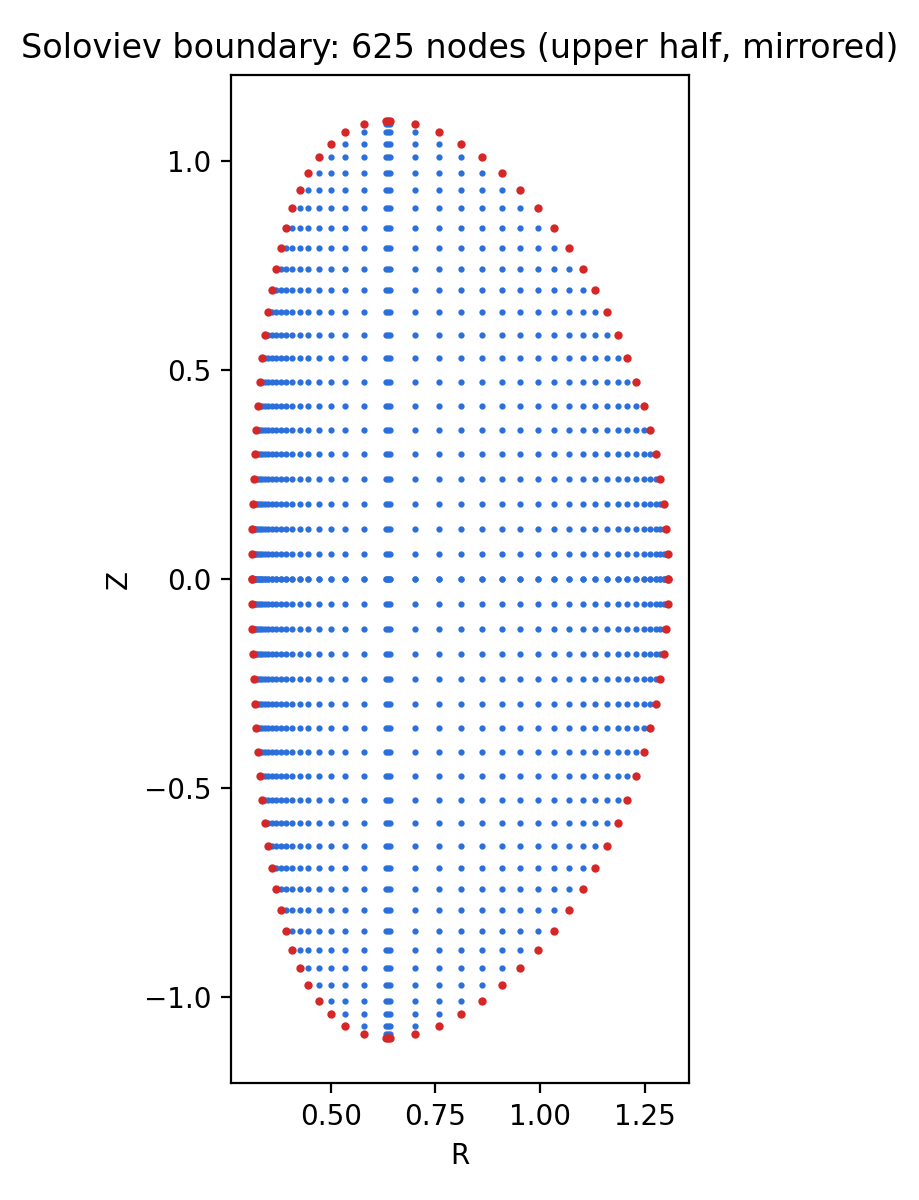
\includegraphics[height=6.2cm]{mesh_soloviev.png}\hspace{1cm}
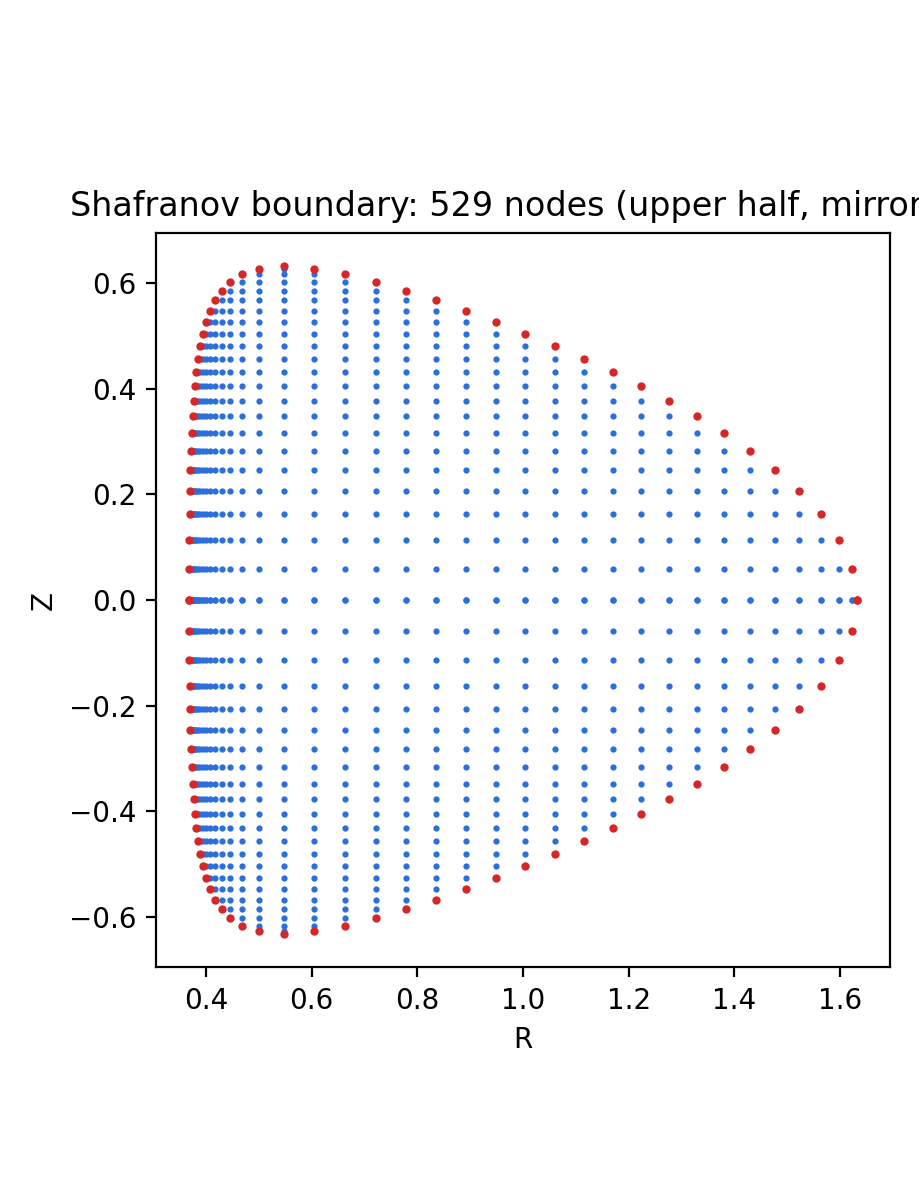
\includegraphics[height=6.2cm]{mesh_shafranov.png}
\caption{Non-homogeneous boundary-fitted meshes (upper half computed, mirrored for display). Red: Dirichlet nodes, blue: interior nodes. Left: Solov'ev contour; right: Shafranov parametric boundary ($\kappa=3$, $\delta=0.8$).}
\label{fig:mesh}
\end{figure}

\subsection{Finite-difference discretisation}

To derive the second-order finite-difference approximation on a non-uniform
3-point stencil, we define
\[
\delta x_i=x_{i+1}-x_i,
\qquad
\delta x_{i-1}=x_i-x_{i-1},
\qquad
\delta x_s=\delta x_i+\delta x_{i-1}.
\]

\textbf{First derivative.}
First, we use second-order Taylor expansions to write
\begin{equation}
    f(x_i+\delta x_i)
    \approx
    f(x_i)
    +f'(x_i)\delta x_i
    +\frac{1}{2}f''(x_i)\delta x_i^2,
\end{equation}
and
\begin{equation}
    f(x_i-\delta x_{i-1})
    \approx
    f(x_i)
    -f'(x_i)\delta x_{i-1}
    +\frac{1}{2}f''(x_i)\delta x_{i-1}^2.
\end{equation}

where t $x_i+\delta x_i=x_{i+1}$ and
$x_i-\delta x_{i-1}=x_{i-1}$. Multiplying the first equation by
$\delta x_{i-1}^2$ and the second by $\delta x_i^2$, and then
subtracting the second equation from the first, yields
\begin{equation}
    \delta x_{i-1}^2 f(x_{i+1})
    -\delta x_i^2 f(x_{i-1})
    =
    f(x_i)
    \left(\delta x_{i-1}^2-\delta x_i^2\right)
    +
    f'(x_i)\delta x_i\delta x_{i-1}\delta x_s.
\end{equation}

Finally, rearranging for $f'(x_i)$ gives
\begin{equation}
    f'(x_i)
    =
    \frac{
        \delta x_{i-1}^2
        \left[f(x_{i+1})-f(x_i)\right]
        -
        \delta x_i^2
        \left[f(x_{i-1})-f(x_i)\right]
    }{
        \delta x_i\delta x_{i-1}\delta x_s
    }.
\end{equation}

\textbf{Second derivative.}
The same procedure is used to obtain the approximation for the second
derivative. Using the same Taylor expansions as above and eliminating
the first derivative before rearranging gives
\begin{equation}
    f''(x_i)
    =
    \frac{
        \delta x_{i-1}
        \left[f(x_{i+1})-f(x_i)\right]
        +
        \delta x_i
        \left[f(x_{i-1})-f(x_i)\right]
    }{
        \frac{1}{2}\delta x_i\delta x_{i-1}\delta x_s
    },
\end{equation}
as in Lopez et al.~\cite{lopez2019}.

Applying these approximations in the $r$-direction for
$\partial_r^2-\tfrac{1}{r}\partial_r$ and in the $z$-direction for
$\partial_z^2$ gives, at an interior node $(i,j)$ with $r=r_i$,
\begin{equation}
    \Dstar\psi\big|_{ij}
    \approx
    c_{R+}\psi_{i+1,j}
    +c_{R-}\psi_{i-1,j}
    +c_{Z+}\psi_{i,j+1}
    +c_{Z-}\psi_{i,j-1}
    +c_0\psi_{ij},
\end{equation}
where
\begin{align*}
    c_{R+}
    &=
    \frac{2}{\delta r_i\delta r_s}
    -
    \frac{\delta r_{i-1}}
    {r\,\delta r_i\delta r_s},
    &
    c_{R-}
    &=
    \frac{2}{\delta r_{i-1}\delta r_s}
    +
    \frac{\delta r_i}
    {r\,\delta r_{i-1}\delta r_s},
    \\[6pt]
    c_{Z+}
    &=
    \frac{2}{\delta z_j\delta z_s},
    &
    c_{Z-}
    &=
    \frac{2}{\delta z_{j-1}\delta z_s},
    \\[6pt]
    c_0
    &=
    -\frac{2}{\delta r_i\delta r_{i-1}}
    +
    \frac{
        \delta r_{i-1}^2-\delta r_i^2
    }{
        r\,\delta r_i\delta r_{i-1}\delta r_s
    }
    -
    \frac{2}{\delta z_j\delta z_{j-1}},
\end{align*}
where
\[
\delta r_s=\delta r_i+\delta r_{i-1},
\qquad
\delta z_s=\delta z_j+\delta z_{j-1}.
\]

This is the same structure as Lopez's Eq.~(14), written for the $\Delta^*$ operator
in the form used in this code.



\paragraph{Boundary conditions.}
\begin{itemize}[nosep]
\item \emph{Midplane} ($z=0$, symmetry): a ghost value $\psi_{i,-1}=\psi_{i,1}$ gives $\partial_z^2\psi|_{z=0}\approx 2(\psi_{i,1}-\psi_{i,0})/\delta z_i^2$.
\item \emph{Boundary}: a node is \emph{Dirichlet} ($\psi=\psi_b$, or simply $1$ in normalised units) if it is on the top row, or has a missing active neighbour in the $r$-direction (inner/outer wall), or a missing neighbour in $z$ (except at the midplane, where the ghost value is used). Dirichlet rows of the matrix are identity rows. Because the grid lines pass through the boundary points in $R$, the radial condition is imposed exactly; a node whose vertical neighbour is missing is, however, assigned the boundary value even though it lies slightly inside the boundary in $z$, which is the main source of the discretisation error discussed in Section~\ref{sec:bench}.
\end{itemize}

\subsection{Sparse linear algebra}
Collecting the active nodes in a single index $k$ gives a linear system $A\bm\psi=\bm b$, where $A\in\mathbb R^{N\times N}$ has at most five non-zeros per row. It is assembled in LIL format (cheap incremental insertion), converted to CSC, and solved with \texttt{scipy.sparse.linalg.spsolve} (sparse LU, SuperLU). Dirichlet rows read $\psi_k=1$ with $b_k=1$; interior rows read $(A\bm\psi)_k=S_k$. For Solov'ev, a single solve ($\approx 0.1$\,s for $N\approx6000$) is enough. The matrix does not depend on $\bm\psi$ in the nonlinear case, only the right-hand side does; for the nonlinear case, the code therefore computes a single \texttt{splu} factorization and reuses it for the subsequent solves. 

\subsection{Picard iteration for the nonlinear case}\label{sec:picarddef}
For the nonlinear source, one step of the iteration is a map $P:\bm\psi\mapsto\bm\psi^{+}$ defined as
\begin{enumerate}[nosep]
\item compute the normalised flux $\pn=(\psi-\psi_{\min})/(\bar\psi_b-\psi_{\min})$ at every node, clipped to $[0,1]$ ($\psi_{\min}$ is the minimum over the grid, $\bar\psi_b$ the mean boundary value);
\item evaluate the right-hand side $b_k=S(r_k,\pn^{(k)})$ at interior nodes ($b_k=1$ on the boundary);
\item solve $A\bm u=\bm b$;
\item renormalise $\bm\psi^+=(\bm u-u_{\min})/(\bar u_b-u_{\min})$.
\end{enumerate}
The iteration (a plain fixed-point or Picard iteration on the nonlinear source, see e.g.\ Jardin~\cite{jardin2010}) is started from $\psi=0$ in the interior and $\psi=1$ on the boundary, $\bm\psi^{k+1}=P(\bm\psi^k)$. A solution of the normalised GS problem is a fixed point $P(\bm\psi)=\bm\psi$, so the stopping test is the \emph{fixed-point residual} $\|P(\bm\psi)-\bm\psi\|/\|\bm\psi\|<10^{-9}$; for every nonlinear run the code reports it, together with $\|P(P(\bm\psi))-\bm\psi\|/\|\bm\psi\|$, and prints a warning if $\bm\psi$ is not a fixed point (and if the iteration looks like a period-two cycle). 
Two structural remarks:
\begin{itemize}[nosep]
\item Because $A$ is linear and step~4 removes any overall factor, \emph{only the ratio $p_0/\alpha$ matters} for the normalised map: scaling $(p_0,\alpha)\to s\,(p_0,\alpha)$ scales $\bm u-\bm 1$ by $s$, which the renormalisation undoes.
\item L\'opez \emph{et al.}\ instead hold the total plasma current and the on-axis pressure fixed by adjusting a coefficient in the $f^2$ profile at every iteration (their Eqs.~(15)--(17)); the code here does not implement that constraint.
\end{itemize}
The geometry is validated at start-up: the Shafranov boundary requires $a<R_0$, since otherwise the plasma crosses $R=0$ where the $1/R$ term of $\Dstar$ is singular.

%=====================================================================
\section{Results}\label{sec:results}
%=====================================================================

\subsection{Benchmark against the Solov'ev solution}\label{sec:bench}
We use the parameters of~\cite{lopez2019}: $B_0=0.5$\,T, $R_0=0.95$, $\kappa_0=2.2$, $q_0=1.1$, $\psi_b=0.09$, on the Solov'ev contour, in mode \texttt{SOLOVIEV\_LINEAR}. Figure~\ref{fig:soloviev} shows the numerical and exact fluxes and their difference for our finest run, $\Delta s=0.006$, which has a $465\times233$ tensor grid in the upper half-plane and $54{,}289$ unknowns there (about $108{,}000$ over the full cross-section). The maximum error is $1.77\times10^{-6}$ and the mean error $4.45\times10^{-7}$, i.e.\ $2\times10^{-5}$ of the peak value of $\psi$. The error is largest around the magnetic axis and decays towards the boundary, where $\psi$ is prescribed.

\begin{figure}[t]
\centering
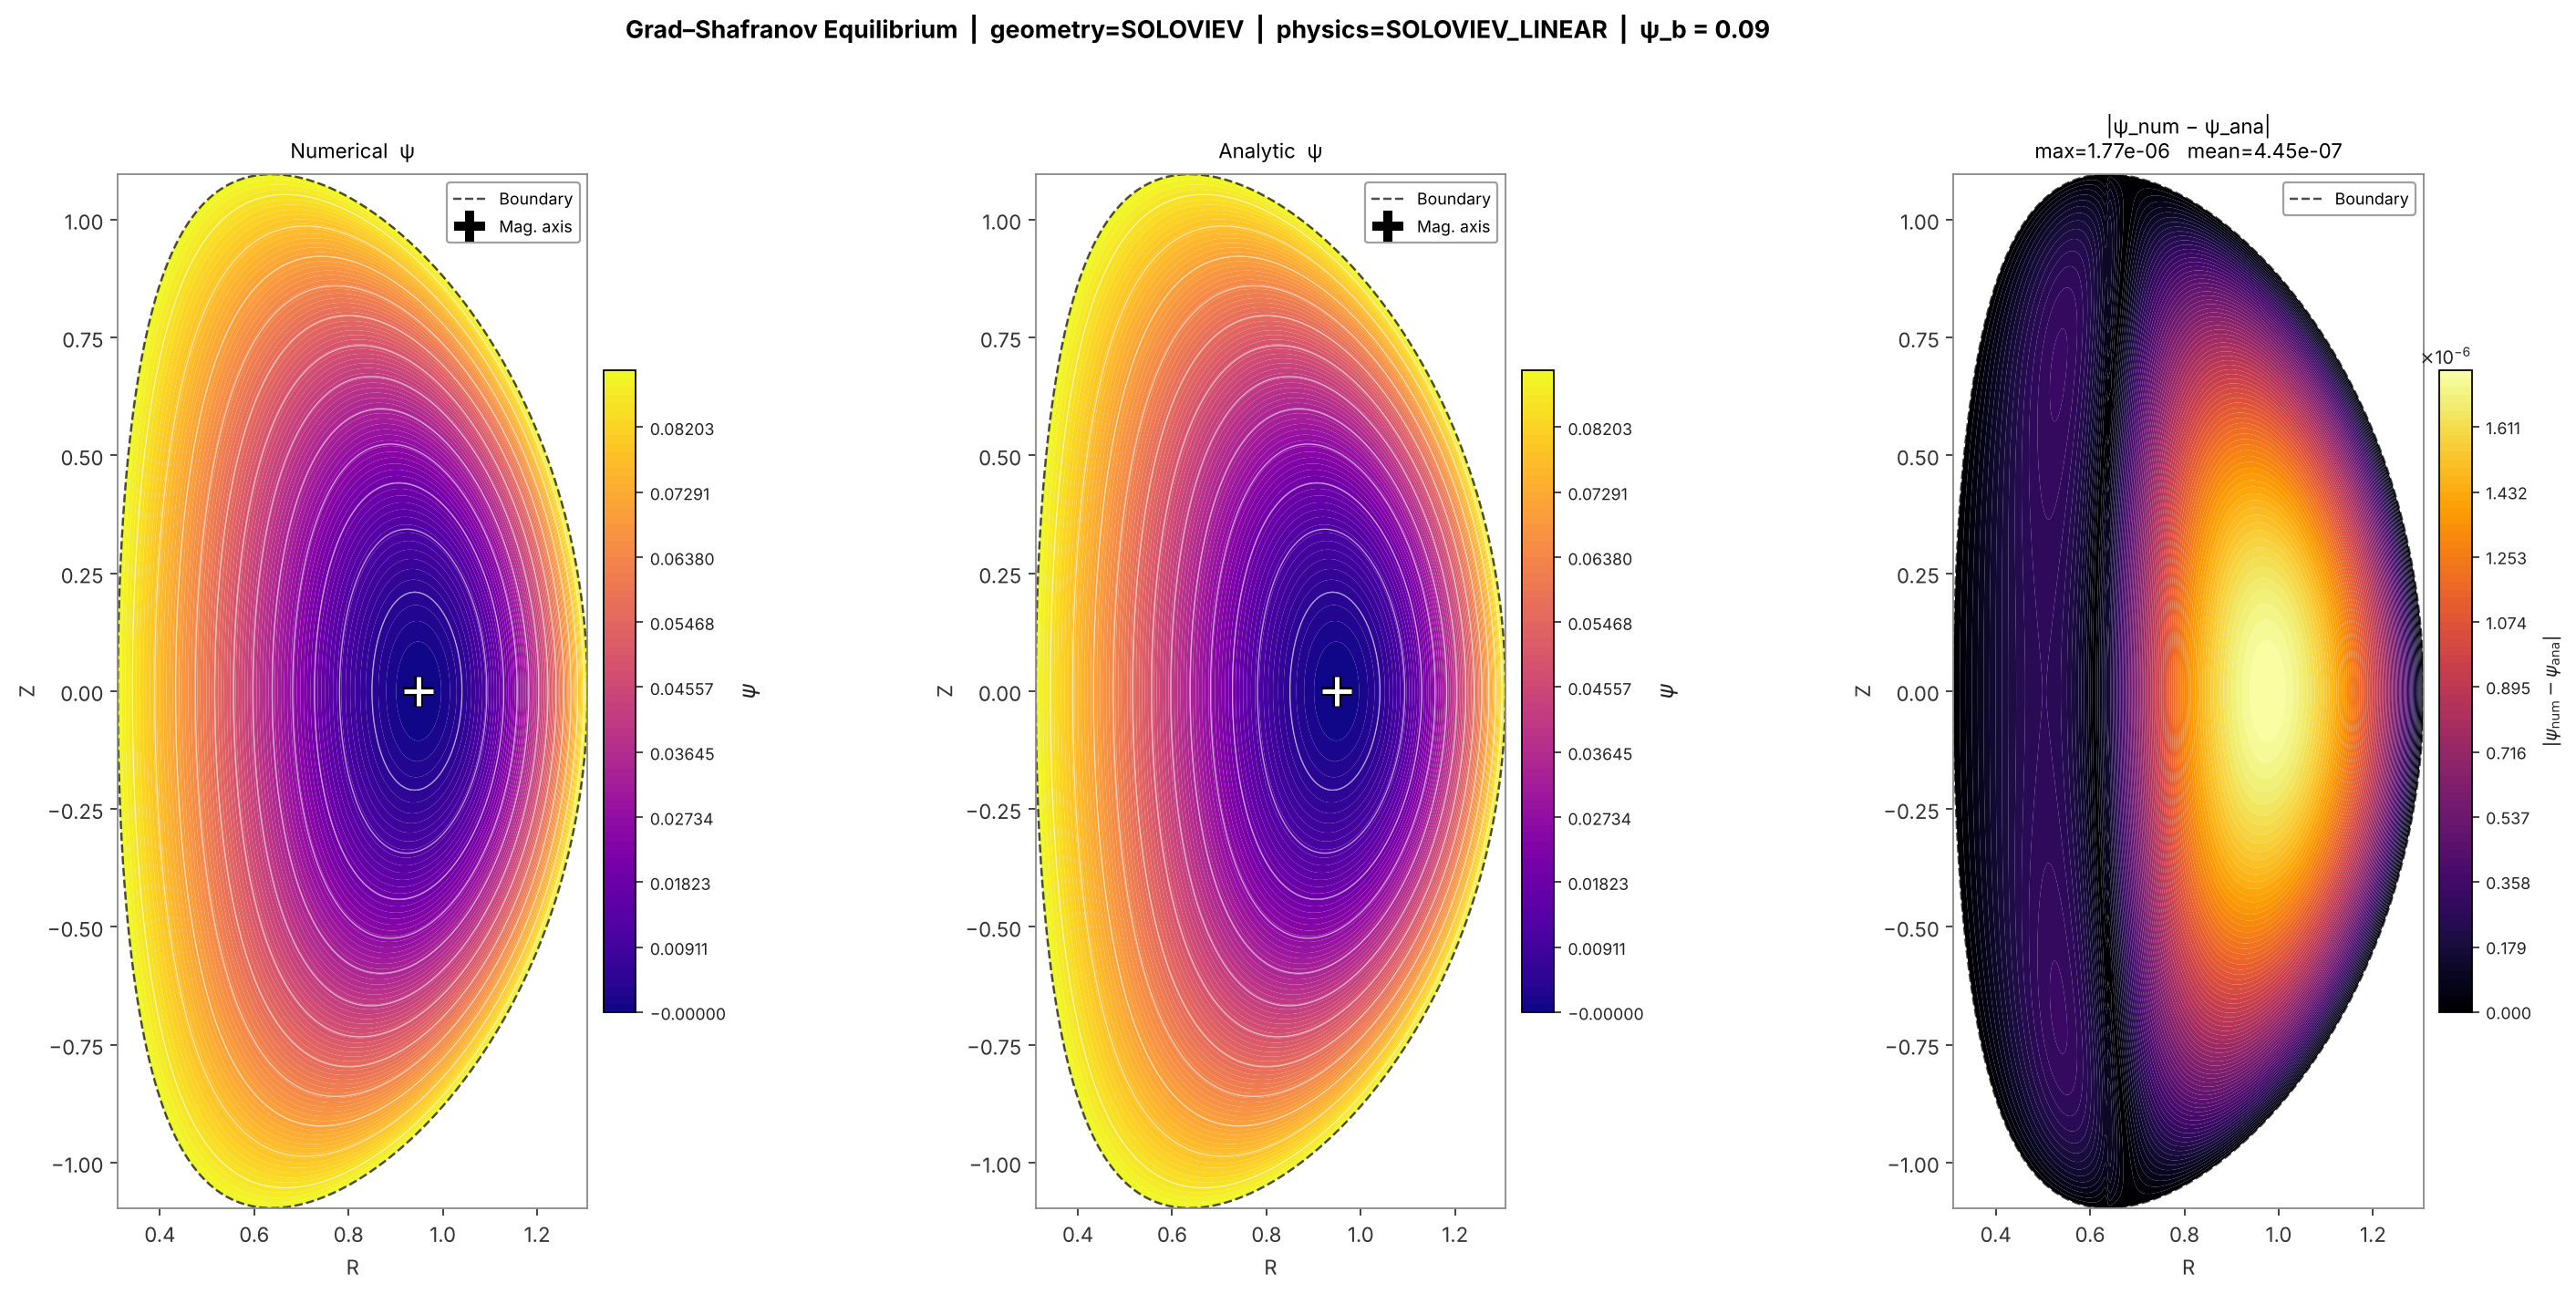
\includegraphics[width=\textwidth]{soloviev_benchmark.png}
\caption{Linear Solov'ev benchmark, $\Delta s=0.006$. Left: numerical $\psi$; middle: analytic $\psi$; right: absolute error.}
\label{fig:soloviev}
\end{figure}

\paragraph{Grid convergence and comparison with L\'opez \emph{et al.}}
Table~\ref{tab:conv} and Figure~\ref{fig:conv} show the error as the boundary step $\Delta s$ is refined. A least-squares fit on the log--log data gives an observed order of $1.90$ (max norm) and $1.83$ (mean), and $1.97$ and $1.93$ over the four finest runs, i.e.\ the second order expected for the stencils. L\'opez \emph{et al.}\ report, for a ``meshgrid of $241\times241$ points'', an error along the $r$ axis that does not exceed $10^{-5}$ (their Fig.~4c). They do not say whether this counts the tensor grid or the active nodes, so we compare with both: our run at $\Delta s=0.012$ has a $233\times233$ tensor grid over the whole domain and a maximum error of $7.0\times10^{-6}$, and our run at $\Delta s=0.0083$ has about $57{,}000$ active nodes over the full cross-section (comparable to $241^2$) and a maximum error of $3.4\times10^{-6}$. In both cases the error lies below their stated bound, although the comparison depends on the way in which nodes are counted and is made only for reference.

\begin{table}[h]
\centering
\caption{Solov'ev grid-convergence study for large $\Delta s$ (error in $\psi$ in the units of $\psi_b=0.09$). $N$ denotes the number of active nodes in the upper half-plane.}
\label{tab:conv}
\begin{tabular}{rrcc}
\toprule
$\Delta s$ & $N$ & max error & mean error\\
\midrule
0.200 & 81   & $1.34\times10^{-3}$ & $2.65\times10^{-4}$\\
0.140 & 144  & $7.34\times10^{-4}$ & $1.45\times10^{-4}$\\
0.100 & 256  & $4.08\times10^{-4}$ & $8.40\times10^{-5}$\\
0.070 & 441  & $2.14\times10^{-4}$ & $4.94\times10^{-5}$\\
0.050 & 841  & $1.11\times10^{-4}$ & $2.61\times10^{-5}$\\
0.035 & 1681 & $5.59\times10^{-5}$ & $1.33\times10^{-5}$\\
0.025 & 3249 & $2.94\times10^{-5}$ & $7.14\times10^{-6}$\\
0.018 & 6241 & $1.53\times10^{-5}$ & $3.72\times10^{-6}$\\
0.012 & 13689 & $6.99\times10^{-6}$ & $1.74\times10^{-6}$\\
0.0083 & 28561 & $3.36\times10^{-6}$ & $8.40\times10^{-7}$\\
0.006  & 54289 & $1.77\times10^{-6}$ & $4.45\times10^{-7}$\\
\bottomrule
\end{tabular}
\end{table}

\begin{figure}[h]
\centering
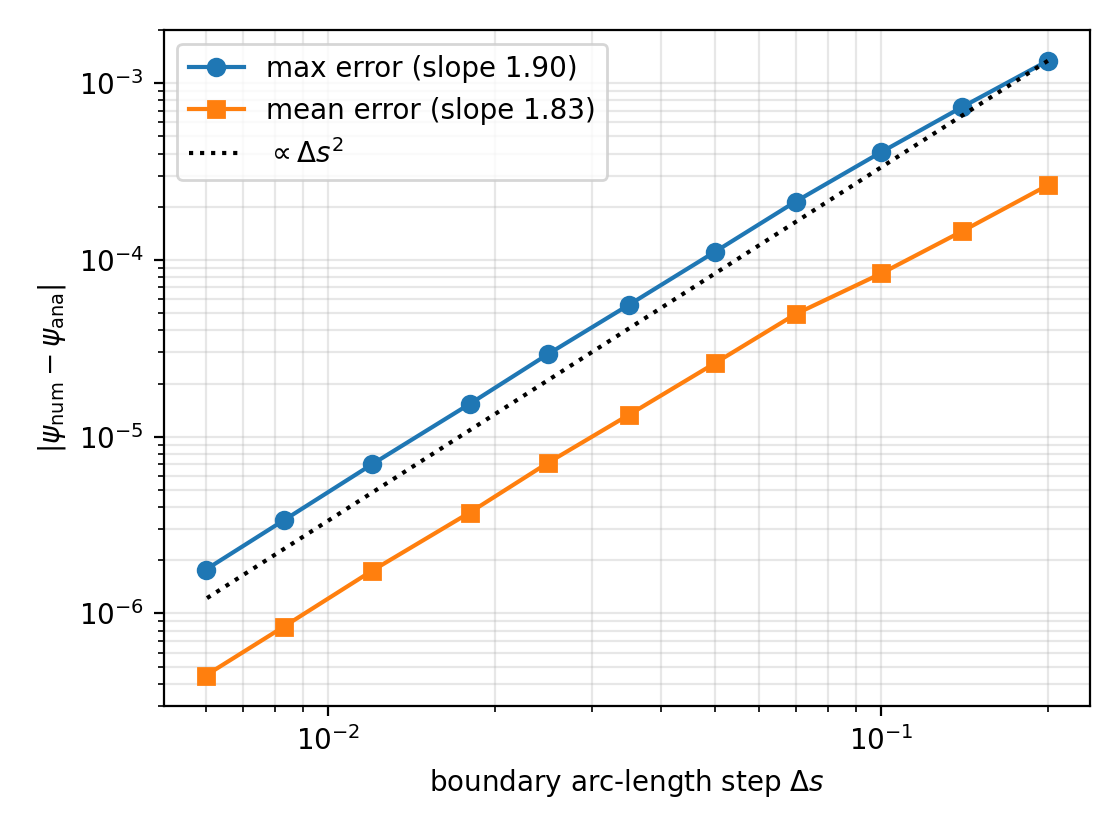
\includegraphics[width=0.55\textwidth]{soloviev_convergence.png}
\caption{Error versus boundary step; dotted: $\propto\Delta s^2$.}
\label{fig:conv}
\end{figure}

\subsection{Validation of the nonlinear code path}\label{sec:nlval}
There is no analytic solution for a generic nonlinear source, so the nonlinear path is validated in two ways (\texttt{scripts/nonlinear\_validation.py}).
\paragraph{Solov'ev through the Picard path.} Running the Picard machinery (\texttt{CUSTOM} source equal to the exact Solov'ev source, plain iteration) must reproduce the analytic solution. It does, converging in 2 iterations (one solve plus one confirming step) to a residual below $10^{-12}$, with maximum errors from $5\times10^{-4}$ at $N=144$ down to $1.7\times10^{-5}$ at $N=3249$, an observed order of $1.9$. The errors are not strictly monotone because the renormalisation uses the discrete minimum of $\psi$, which exceeds the true axis value by an amount that varies with the (non-nested) mesh.
\paragraph{Grid convergence of a nonlinear case.} For the ITER-like boundary with baseline profiles we track the amplitude functional $C=1-u_{\min}$ (the flux difference between boundary and axis in the unnormalised solve at the fixed point) for $N=144$ up to $6889$. It converges, from $0.16780$ to $0.16729$, with a fit $C(\Delta s)=C_\infty+c\,\Delta s^{p}$ giving $C_\infty=0.16723$ and $p\approx1.2$; the plain iteration needs $27$--$28$ iterations at every resolution and the residual is $<4\times10^{-13}$ throughout. The observed order is closer to one than to two, consistent with the first-order treatment of the vertical boundary condition and with non-nested meshes. We therefore claim convergence, but not second-order accuracy, for the nonlinear solutions.

\subsection{Nonlinear equilibria: profiles and shapes}\label{sec:profiles}
We use the Shafranov boundary with $R_0=0.95$, $a=0.6$ ($a/R_0=0.63$), $\Delta s=0.05$, and plain Picard iteration. Baseline exponents are $(s_{p1},s_{p2})=(2,2)$, $(s_{f1},s_{f2})=(2,1)$ and $p_0=\alpha=1$. We first vary the boundary shape, then the profiles at the ITER-like shape $\kappa=1.7$, $\delta=0.33$. Table~\ref{tab:nl} lists the iterations needed, the fixed-point residual, the position of the magnetic axis and its displacement from the geometric centre of the midplane chord, normalised by its half-width. The axis is computed by parabolic interpolation through the three midplane nodes around the minimum.

\begin{table}[h]
\centering
\caption{Nonlinear cases (plain Picard). All reach a true fixed point of $P$.}
\label{tab:nl}
\small
\begin{tabular}{llrrcccc}
\toprule
case & $(\kappa,\delta)$ & $N$ & iter. & $\|P\bm\psi-\bm\psi\|/\|\bm\psi\|$ & $R_{\rm axis}$ & shift/half-width\\
\midrule
circular                          & (1.0, 0.00) & 441  & 22 & $1.9\times10^{-11}$ & 1.174 & $+0.275$\\
ITER-like (baseline)              & (1.7, 0.33) & 961  & 23 & $1.6\times10^{-11}$ & 1.152 & $+0.240$\\
strong D                          & (3.0, 0.80) & 2209 & 30 & $2.6\times10^{-11}$ & 1.151 & $+0.238$\\
\midrule
peaked $p'$, $(s_{p1},s_{p2})=(2,4)$      & (1.7, 0.33) & 961 & 26 & $2.3\times10^{-11}$ & 1.149 & $+0.236$\\
broad $p'$, $FF'$, $(4,1)$ and $(4,1)$    & (1.7, 0.33) & 961 & 15 & $1.3\times10^{-11}$ & 1.147 & $+0.232$\\
current-driven, $p_0{=}0.2,\ \alpha{=}2$  & (1.7, 0.33) & 961 & 20 & $1.4\times10^{-11}$ & 1.078 & $+0.124$\\
pressure-driven, $p_0{=}3,\ \alpha{=}0.3$ & (1.7, 0.33) & 961 & 25 & $3.7\times10^{-11}$ & 1.189 & $+0.300$\\
\bottomrule
\end{tabular}
\end{table}

\begin{figure}[t]
\centering
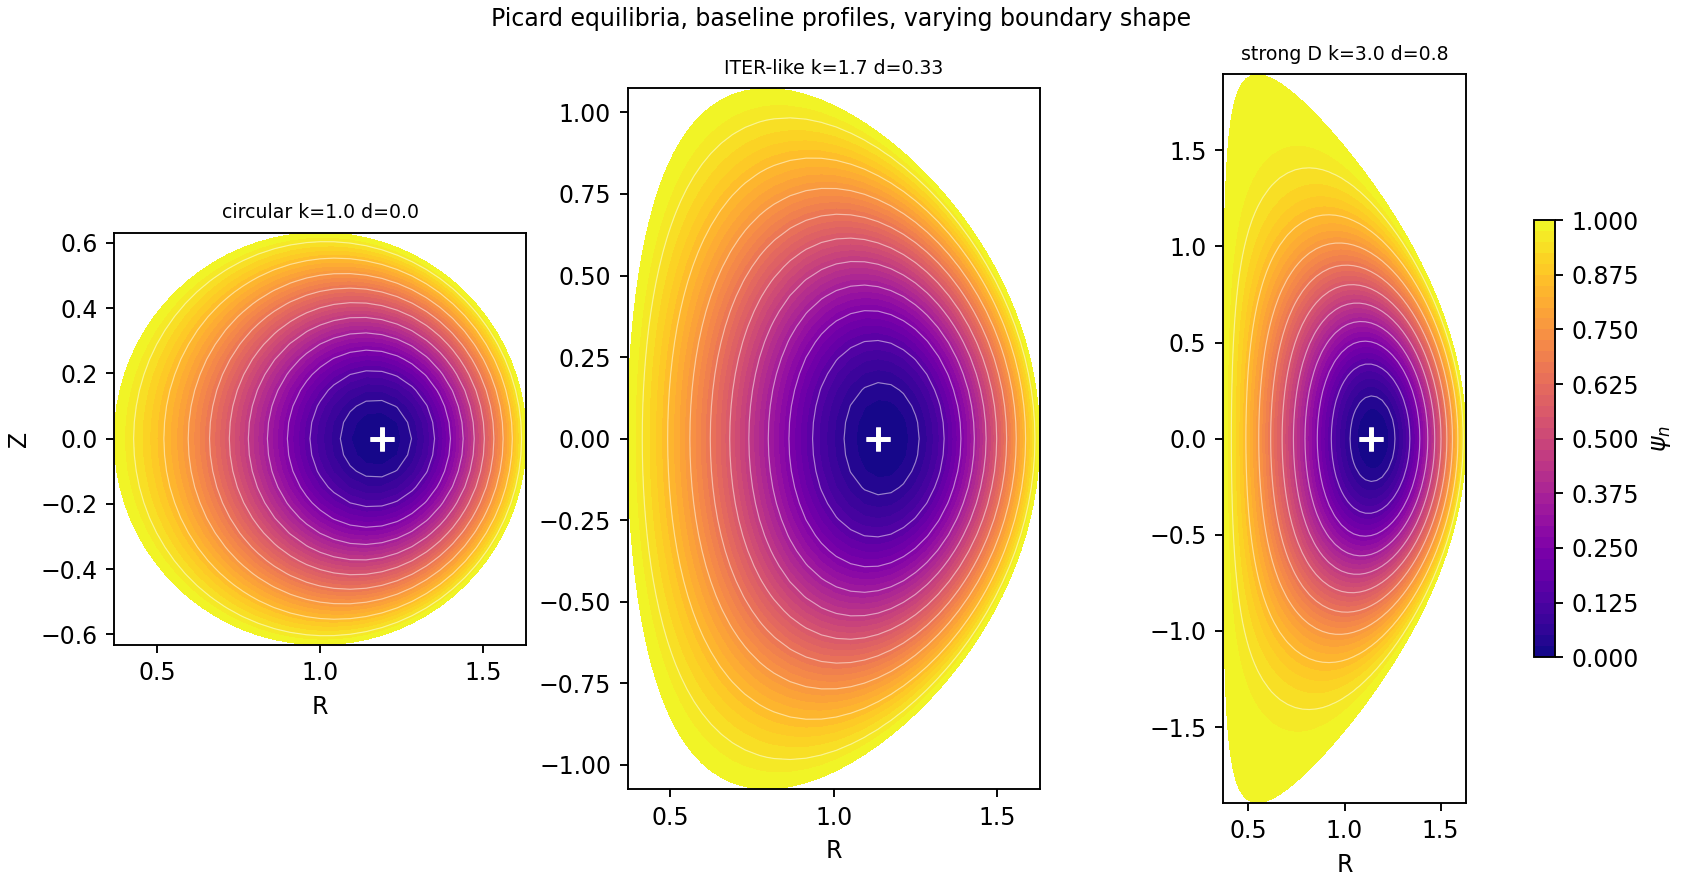
\includegraphics[width=\textwidth]{nonlinear_shapes.png}
\caption{Flux surfaces ($\pn$ contours; white $+$: magnetic axis) at the baseline profiles for three boundary shapes: circular, ITER-like, strong D.}
\label{fig:shapes}
\end{figure}

\begin{figure}[t]
\centering
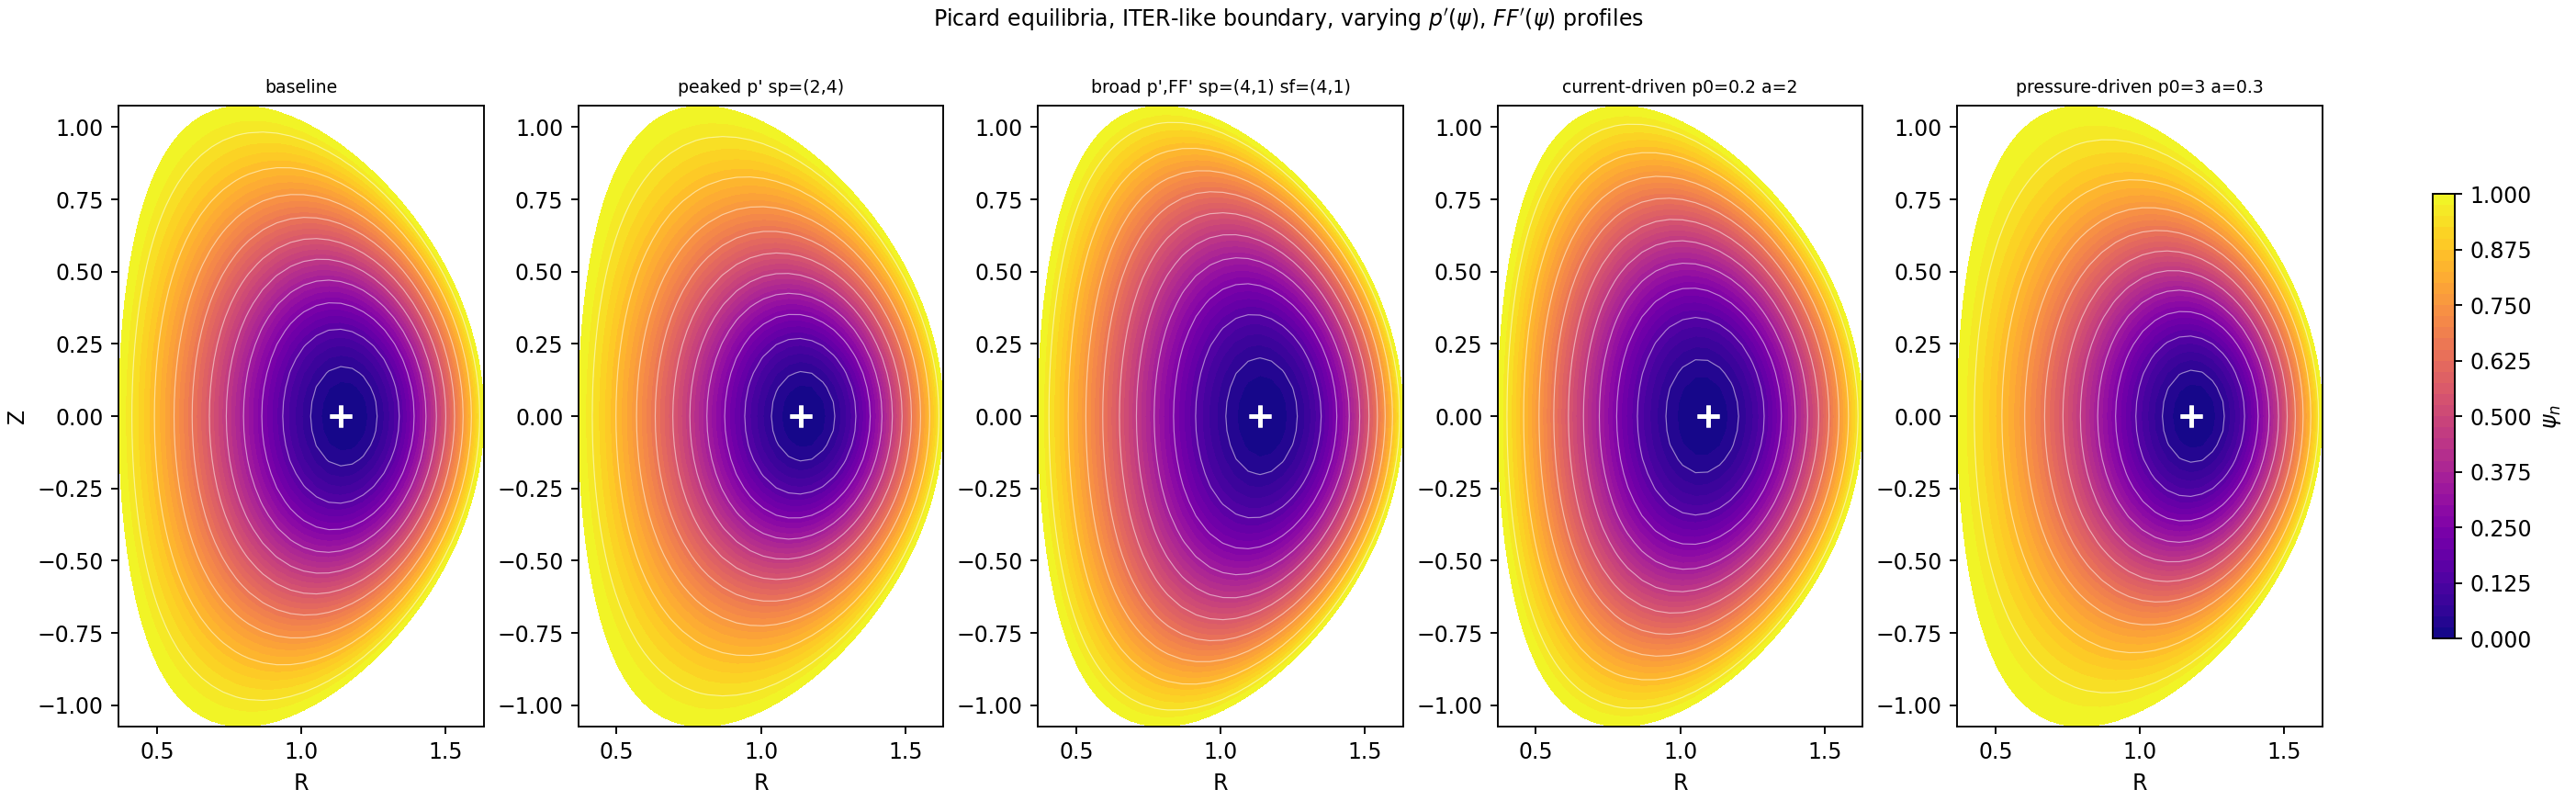
\includegraphics[width=\textwidth]{nonlinear_profiles.png}
\caption{Flux surfaces at the ITER-like boundary for five choices of the profiles.}
\label{fig:profiles}
\end{figure}

\begin{figure}[t]
\centering
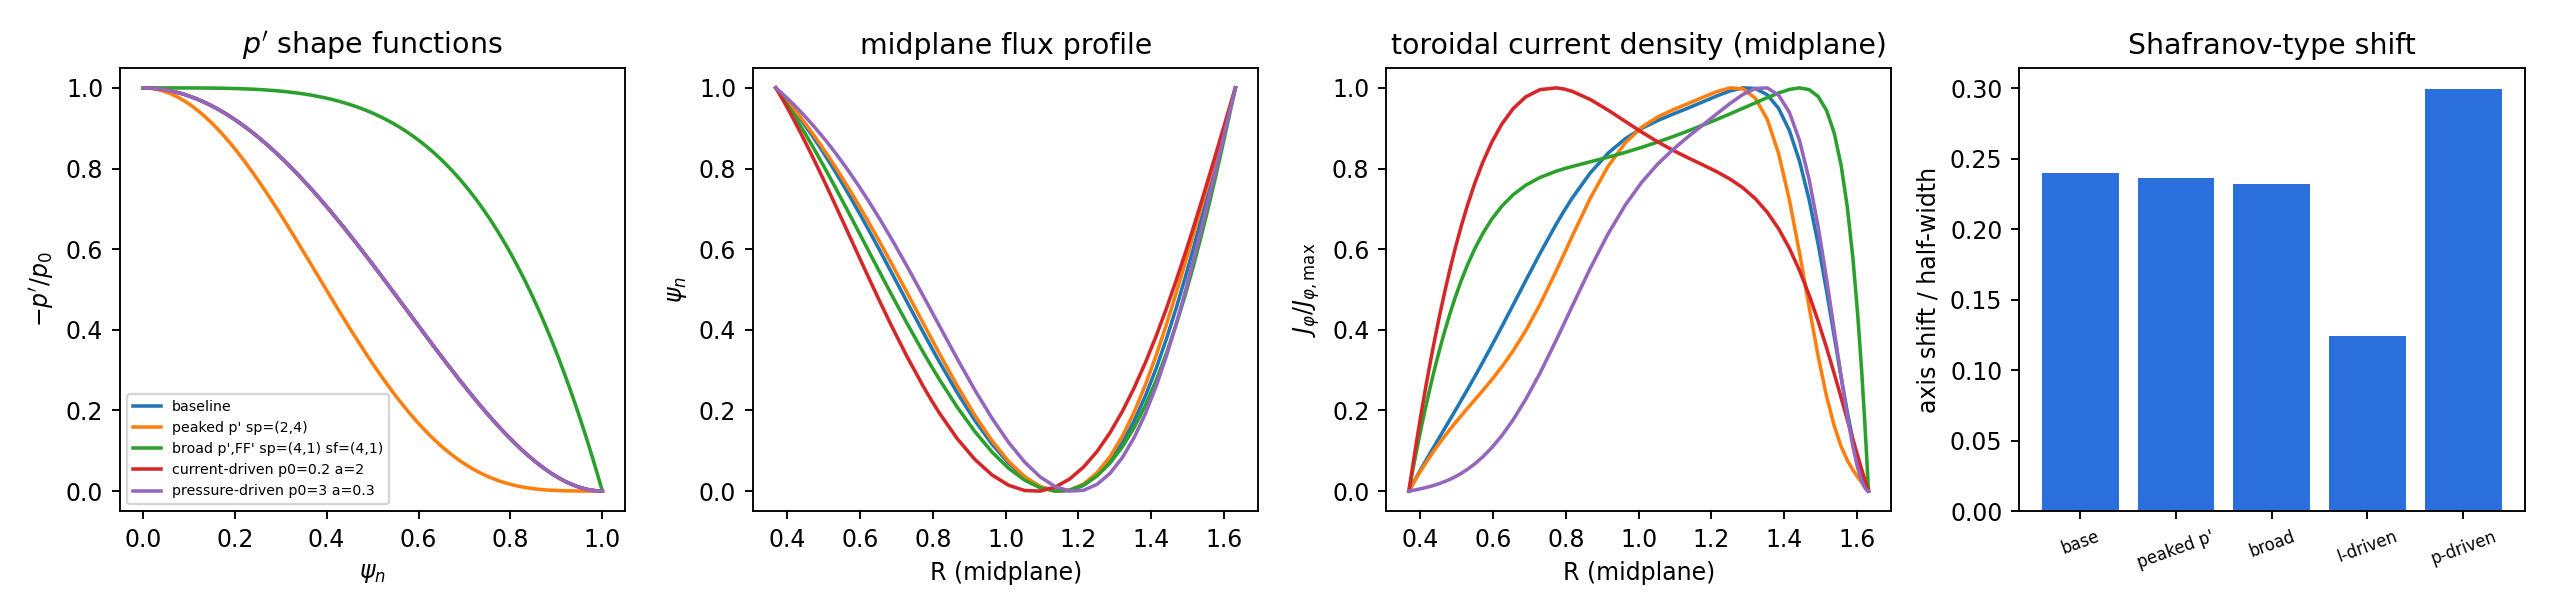
\includegraphics[width=\textwidth]{nonlinear_profile_diagnostics.png}
\caption{Left to right: shape of $-p'$; midplane flux profile; midplane toroidal current density $J_\varphi\propto S/R$ (each case normalised to its maximum); normalised axis shift.}
\label{fig:diag}
\end{figure}

\paragraph{Observations}
\begin{itemize}[nosep]
\item \emph{The axis shifts outward even for a circular boundary.} The circular case is not symmetric under $R\to2R_0-R$. At first glance this may be surprising, but in fact it is expected because the $\Delta^*$ operator contains a $1/R$ term due to the toroidal geometry. The axis sits at $+0.28$ half-widths outward of the geometric centre. This is the Shafranov shift, as the flux surfaces are compressed on the outboard side and the axis moves outward relative to the centre of the boundary. Increasing the shaping to $\kappa=1.7,\delta=0.33$ or to $\kappa=3,\delta=0.8$ changes the normalised shift only slightly ($0.275\to0.240\to0.238$), while the surfaces follow the D-shape (Fig.~\ref{fig:shapes}).
\item \emph{The shift is controlled by the pressure-to-current ratio.} The shift is in fact not strongly controlled by the peaking of the $p'$ or $FF'$ functions. At fixed ratio $p_0/\alpha=1$, changing the exponents (peaked, baseline or broad $p'$ and $FF'$) moves the shift only between $0.232$ and $0.240$. Rather, it is controlled by their ratio: $p_0/\alpha=0.1$ gives a shift of $0.124$ and $p_0/\alpha=10$ gives $0.300$, a factor $2.4$. This is consistent with the dependence of the Shafranov shift on poloidal beta, as more pressure support relative to the poloidal-field-producing current pushes the axis outward.
\item \emph{The current density profile follows suit.} Since $\mu_0J_\varphi=-S/R$ and $S=-\mu_0R^2p'-FF'$, the current density is
\begin{equation*}
J_\varphi\propto R\,(-p')+\frac{1}{R}\,(-FF'),
\end{equation*}
where the pressure term grows with $R$ and the toroidal-field term decays with it. The midplane current density therefore peaks outboard of the axis for pressure-driven profiles and inboard for toroidal-field-driven ones (Fig.~\ref{fig:diag}, third panel).
\item \emph{Cost.} All cases converge to residuals of $10^{-11}$ in $15$--$30$ plain Picard iterations; broader profiles converge fastest (spectral radius $0.22$ versus $0.44$ for the peaked $p'$; Table~\ref{tab:spec}).
\end{itemize}

%=====================================================================
\section{Convergence of the Picard iteration}\label{sec:picard}
%=====================================================================

\subsection{Linear stability}
Let $P$ be the one-step Picard map of Section~\ref{sec:picarddef}, $\bm\psi^*$ a fixed point and $L=\partial P/\partial\bm\psi|_{\bm\psi^*}$ its Jacobian. Near $\bm\psi^*$ the error evolves as $\bm e^{k+1}\approx L\bm e^k$, so plain Picard converges if and only if the spectral radius $\rho(L)<1$, with asymptotic rate $\rho(L)$ per iteration; reducing the residual by a factor $\varepsilon$ takes about $\ln\varepsilon/\ln\rho(L)$ iterations. 
We build $L$ column by column by central differences, 
$$L\bm e_j\approx\frac{P(\bm\psi^*+\eta\bm e_j)-P(\bm\psi^*-\eta\bm e_j)}{2\eta}$$ with $\eta=10^{-6}\|\bm\psi^*\|$. For smaller grids (up to $N\approx10^3$), we diagonalise it densely. For larger grids the code can instead estimate the leading eigenvalues matrix-free with \texttt{scipy.sparse.linalg.eigs} (\texttt{SPECTRAL\_ANALYSIS}).

\subsection{Measurements}
All numbers below come from \texttt{scripts/spectral\_study.py} (output in \texttt{results/spectral\_study.json}).

\begin{figure}[t]
\centering
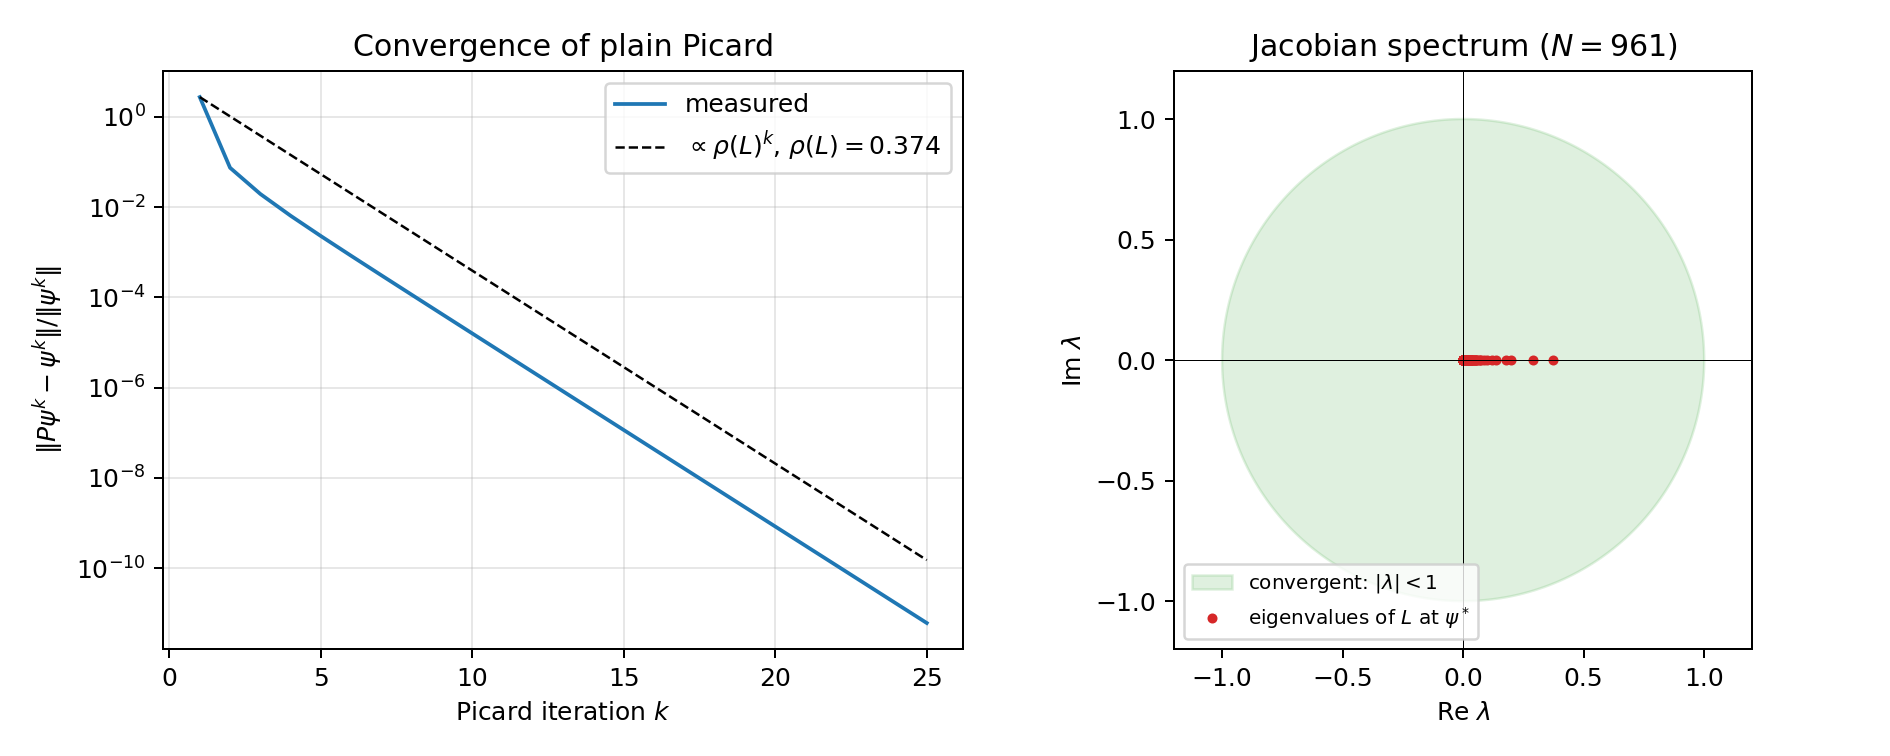
\includegraphics[width=\textwidth]{picard_spectral_study.png}
\caption{Left: fixed-point residual of plain Picard (ITER-like boundary, baseline profiles, $N=961$) and the decay $\rho(L)^k$ predicted by the spectral radius. Right: eigenvalues of the Picard Jacobian $L$ at the fixed point against the unit disc.}
\label{fig:spectral}
\end{figure}

\paragraph{Main case ($N=961$).} Plain Picard reaches a residual of $10^{-11}$ in $25$ iterations. The spectrum of $L$ at the fixed point is real and non-negative, $\lambda\in[0,0.374]$ (largest imaginary part $2\times10^{-6}$), so $\rho(L)=0.374$ and the predicted number of iterations is $\ln10^{-11}/\ln0.374=25.7$, matching the observed $25$ (Fig.~\ref{fig:spectral}).

\begin{table}[h]
\centering
\caption{Plain-Picard iterations (to a residual of $10^{-11}$) and spectral radius of $L$ at the fixed point, dense Jacobian. In every case the spectrum is real and non-negative to within $4\times10^{-4}$ in imaginary part.}
\label{tab:spec}
\small
\begin{tabular}{lrcc}
\toprule
case & $N$ & iterations & $\rho(L)$\\
\midrule
ITER-like, baseline              & 484 & 25 & 0.380\\
circular                         & 225 & 24 & 0.374\\
strong D $(3.0,0.8)$             & 576 & 33 & 0.484\\
pressure-driven, $p_0/\alpha=10$ & 484 & 28 & 0.420\\
current-driven, $p_0/\alpha=0.1$ & 484 & 22 & 0.316\\
broad profiles                   & 484 & 17 & 0.219\\
peaked $p'$                      & 484 & 29 & 0.437\\
\bottomrule
\end{tabular}
\end{table}

\paragraph{Reading.} With peaked-current profiles the Jacobian has a real, non-negative spectrum inside $[0,0.5)$, so plain Picard converges monotonically with rate $0.22$--$0.48$ in all seven configurations tested, and $\rho(L)$ predicts the iteration count well. Broader profiles converge fastest; strong shaping and peaked $p'$ slowest. We have not tested hollow-current, high-beta or very strongly shaped profiles, where the spectrum could look different.


\section{Conclusion}\label{sec:conclusion}
We have built a fixed-boundary Grad--Shafranov solver on a boundary-fitted, non-homogeneous mesh, following the scheme of L\'opez \emph{et al.}~\cite{lopez2019}, and extended it from their linear Solov'ev setting to the general nonlinear case with arbitrary $p'(\psi)$ and $FF'(\psi)$. The linear solver reproduces the analytic Solov'ev equilibrium at an observed order of about $1.9$, with a maximum error of $7\times10^{-6}$ on a $233\times233$ grid, below the $10^{-5}$ bound reported by L\'opez \emph{et al.}\ at comparable resolution. The nonlinear path, a Picard iteration with the fixed-point residual as stopping criterion and a single sparse LU factorisation reused across iterations, reproduces the Solov'ev solution when fed the Solov'ev source. On a nonlinear case it converges under mesh refinement, at roughly first order for the quantity we monitored. Across seven combinations of boundary shape and profile it reaches residuals of $10^{-11}$ in $15$--$33$ iterations, a count that the spectral radius of the Picard Jacobian, real and positive with $\rho(L)\in[0.22,0.48]$, predicts well. The equilibria show the expected outward Shafranov shift of the magnetic axis, controlled mainly by the ratio of the pressure and toroidal-field amplitudes rather than by the peaking of the profiles.

The solver has clear limits, which point to natural extensions. Its boundary is prescribed rather than computed, so a free-boundary version would be needed to capture the plasma's response to coil currents and to locate the separatrix and X-points. It also does not hold the total plasma current and axis pressure fixed as in~\cite{lopez2019}, and it could be interesting to explore how implementing that constraint affects accuracy and convergence. On the numerical side, an acceleration scheme such as Anderson's~\cite{anderson1965} could help for more demanding profiles, such as hollow-current or higher-beta ones, which we have not tested. Finally, the same matrix machinery could support the inverse problem of Section~\ref{sec:context}, fitting $p'(\psi)$ and $FF'(\psi)$ to measurements, which would turn the solver from a tool for exploring profile scenarios into one for reconstructing equilibria from real-world tokamak data.
%=====================================================================
\section*{Acknowledgements}
This work was carried out as a project for the Classical Electrodynamics course at \'Ecole Polytechnique, within a group in which each member worked on a different part of the problem and ended up with their own version of the solver. I thank Jacques Stefani for presenting me with the Picard iteration method from Jardin's book. I also thank Prof. Arnaud Couairon for the regular meetings throughout the project in which we discussed its progress.

\appendix
\section{Derivation of the Grad--Shafranov equation}\label{app:derivation}
%=====================================================================
\emph{This derivation follows the approach of Ben Dudson's lecture series ``Plasma fluid theory''~\cite{dudson}.} 

There are three main steps to the derivation, using 
\begin{itemize}
    \item $\mathbf{B}=\nabla \times \mathbf{A}$ (Basic vector potential)
    \item $\mu_0\mathbf{\mathbf{J}}=\nabla \times \mathbf{B}$ (Maxwell Ampère - we study static equilibrium so the displacement current is irrelevant)
    \item $\mathbf{J} \times\mathbf{B}=\nabla p$ (MHD)
\end{itemize}
The main assumption we use is that of symmetry about the axis, whereby 
$$\frac{\partial}{\partial\phi}=0$$
for all scalar fields considered. Note, however, that the cylindrical basis vectors $\hat{\boldsymbol{\phi}}$ and $\mathbf{\hat{r}}$ both retain their dependency on $\phi$, and we still have 
$$\partial_\phi\mathbf{\hat{r}}=\hat{\boldsymbol{\phi}} \quad \& \quad\partial_\phi\hat{\boldsymbol{\phi}}=-\mathbf{\hat{r}}$$
This distinction is subtle, and important to keep track of as it leads to the appearance of the elliptic operator $\Delta^*$ which is so central to this problem. As stated, we study static equilibria so $\partial_t\equiv 0$.

\subsection{Step I: Vector potential}
    Consider a cylindrical geometry with basis $(r, \phi,z)$. Using symmetry about the axis ($\partial/\partial\phi =0$) the first equation writes
    $$\mathbf{B}=-\frac{1}{r}\frac{\partial}{\partial z}(rA_{\phi})\hat{\mathbf{r}}+\frac{1}{r}\frac{\partial}{\partial r}(rA_{\phi})\hat{\mathbf{z}}+B_\phi \hat{\boldsymbol{\phi}}$$
    
    Where 
    $$B_\phi =\frac{\partial}{\partial z}A_r-\frac{\partial}{\partial r}A_z$$
    
    Define the poloidal flux function
    $$\psi:=rA_\phi$$
    Then 
    $$\begin{aligned}
        \mathbf{B}&=-\frac{1}{r}\frac{\partial\psi}{\partial z}\hat{\mathbf{r}}+\frac{1}{r}\frac{\partial \psi}{\partial r}\hat{\mathbf{z}}+B_\phi \hat{\boldsymbol{\phi}}\\
        &=\boxed{\frac{1}{r} \nabla\psi\times\hat{\boldsymbol{\phi}}+B_\phi \hat{\boldsymbol{\phi}}}
    \end{aligned}
    $$

    Now imagine a poloidal plane. The purpose of defining $\psi$ as above is that the poloidal part of B, $\mathbf{B_\rho}$, is tangential to surfaces of constant $\psi$. To show this, notice first that $\nabla\psi$ is perpendicular to such surfaces, because the directional derivative along the tangent to the surface is zero. Mathematically, if $\mathbf{u}$ is a tangent to a surface of constant $\psi$, then at that point 
    $$\frac{\partial}{\partial \mathbf{u}}\psi=0 \iff \mathbf{u} \cdot \nabla\psi=0 \iff \mathbf{u} \perp \nabla\psi$$
    From the expression for B above, one checks $\nabla\psi\cdot\mathbf{B}=0$ so that $\mathbf{B}$ is also perpendicular to $\nabla\psi$, we conclude that it is co-linear to $\mathbf{u}$. We have thus established that field lines of B are surfaces where $\psi$ is constant.

\subsection{Step II: Maxwell-Ampère}
    Next, we use Maxwell Ampère to find an expression for the current. In order to do so, we compute the curl of B.
    $$\begin{aligned}
        \nabla\times\mathbf{B}&=\nabla\times\left(\frac{1}{r}\nabla\psi\times\hat{\boldsymbol{\phi}}\right)+\nabla\times(B_\phi\hat{\boldsymbol{\phi}})    \end{aligned}
    $$
    Compute the two parts separately. First, using the vector calculus expansion for $\nabla\times(\mathbf{X\times\mathbf{Y)}}$, 
    $$\begin{aligned}
        \nabla\times(\frac{1}{r}\nabla\psi\times\hat{\boldsymbol{\phi}}) &= \underbrace{(\nabla \cdot \hat{\boldsymbol{\phi}})}_{0}\frac{1}{r}\nabla\psi +\underbrace{(\hat{\boldsymbol{\phi}}\cdot\nabla)}_{\frac{1}{r}\frac{\partial}{\partial \phi}}\frac{1}{r}\nabla\psi - \underbrace{\left(\frac{1}{r}\nabla\psi \cdot \nabla\right)\hat{\boldsymbol{\phi}}}_{0} - \left(\nabla\cdot \frac{1}{r} \nabla\psi\right)\hat{\boldsymbol{\phi}}
        \\
        &= \frac{1}{r}\frac{\partial}{\partial\phi}\left(\frac{1}{r}\frac{\partial\psi}{\partial r} \mathbf{\hat{r}} + \frac{1}{r} \frac{\partial\psi}{\partial z}\mathbf{\hat{z}}\right)- \left(\nabla\cdot (\frac{1}{r} \nabla\psi)\right)\boldsymbol{\hat{\phi}} \\
        &= \frac{1}{r^2}\frac{\partial\psi}{\partial r} \frac{\partial\mathbf{\hat{r}}}{\partial\phi} + \frac{1}{r^2} \frac{\partial\psi}{\partial z}\frac{\partial\mathbf{\hat{z}}}{\partial\phi} - \left(\nabla\cdot (\frac{1}{r} \nabla\psi)\right)\boldsymbol{\hat{\phi}}\\
        &= \left(\frac{1}{r^2}\frac{\partial\psi}{\partial r} - \nabla\cdot (\frac{1}{r} \nabla\psi)\right)\boldsymbol{\hat{\phi}} \\
        &= \left[\frac{1}{r^2}\frac{\partial\psi}{\partial r} - \left(\nabla(\frac{1}{r}) \cdot \nabla\psi + \frac{1}{r} \nabla^2 \psi \right)\right] \hat{\boldsymbol{\phi}}\\
        &= \left(\frac{2}{r^2}\frac{\partial\psi}{\partial r}-\frac{1}{r}\frac{\partial^2\psi}{\partial z^2}-\frac{1}{r^2}\frac{\partial\psi}{\partial r}-\frac{\partial^2\psi}{\partial r^2}\right)\hat{\boldsymbol{\phi}} \\
        &= -\frac{1}{r}\left(\frac{\partial^2\psi}{\partial r^2}-\frac{1}{r}\frac{\partial\psi}{\partial r}+\frac{\partial^2\psi}{\partial z^2}\right)\hat{\boldsymbol{\phi}} \\
        &= -\frac{1}{r} \Delta ^* \psi \hat{\boldsymbol{\phi}}
    \end{aligned}
    $$

    Second, multiply and divide by $r$ to write 
    $$
    \begin{aligned}
        \nabla \times(B_\phi \hat{\boldsymbol{\phi}}) &= \nabla\times(rB_\phi\frac{\hat{\boldsymbol{\phi}}}{r}) \\
        &= rB_\phi\underbrace{(\nabla\times\frac{\hat{\boldsymbol{\phi}}}{r})}_{0}+\nabla(rB_\phi)\times\frac{\hat{\boldsymbol{\phi}}}{r} \\
        &= \nabla(rB_\phi)\times\frac{\hat{\boldsymbol{\phi}}}{r}
    \end{aligned}
    $$
    where the first term is zero from the equation for curl in cylindrical coordinates.
    Combining, we get
    $$\begin{aligned}
        \mu_0\mathbf{J}&=\underbrace{\nabla(rB_\phi)\times\frac{\hat{\boldsymbol{\phi}}}{r}}_{\text{poloidal current}}+ \underbrace{\left(-\frac{1}{r}\Delta^*\psi\right)}_{\mu_0J_\phi}\,\hat{\boldsymbol{\phi}}
    \end{aligned}
    $$
    
\subsection{Step III: Using MHD stability equation}
    We recall that the axi-symmetry assumption implies that the toroidal derivative of the pressure is null, and thus that the pressure gradient has no toroidal component. Mathematically, this can be written as $\nabla p \cdot \hat{\boldsymbol{\phi}}=0$. With this assumption in mind, we now turn to the MHD equilibrium condition. 

    \subsubsection{Intermediate calculations}
    Some intermediate steps are necessary before we can apply the MHD force balance in full, namely we must define the function $f$ and show that both $p$ and $f$ are functions of $\psi$.
    
    \paragraph{Showing $p=p(\psi)$}: From the MHD equation,
    $$\mathbf{J}\times\mathbf{B}=\nabla p \implies \mathbf{B}\cdot\nabla p =0$$
    Plugging back in the expression for B,
    $$\begin{aligned}
        \nabla p \cdot \mathbf{B}&=\nabla p \cdot \left(\frac{1}{r} \nabla\psi\times\hat{\boldsymbol{\phi}}+B_\phi \hat{\boldsymbol{\phi}}\right) \\
        &= \nabla p \cdot \left(\frac{1}{r} \nabla\psi\times\hat{\boldsymbol{\phi}}\right) 
    \end{aligned}
    $$
    so that, using the triple product and multiplying through by $r$, we obtain
    $$(\nabla \psi \times \nabla p) \cdot \hat{\boldsymbol{\phi}}=0$$
    Computing the cross product,
    $$ \frac{\partial \psi}{\partial r} \frac{\partial p}{\partial z} - \frac{\partial \psi}{\partial z}\frac{\partial p}{\partial r}=0$$
    
    Thus
    $$\nabla p \propto \nabla \psi$$ 
    This means that $\psi$ and $p$ have the same level sets, or surfaces of constant value. We deduce that 

    $$p=h \circ\psi$$

    for some function $h$. Written more concisely, $p=p(\psi)$, and 
    $$\nabla p = \frac{d p}{d\psi}\,\nabla\psi$$

    \paragraph{Building the F function and showing $f=f(\psi)$}: The same way from the MHD equation, we get 
    $$\begin{aligned}
        \nabla p\cdot\mathbf{J}=0 &\implies \nabla p \cdot \left[\nabla(rB_\phi)\times\frac{\hat{\boldsymbol{\phi}}}{r}+ \left(-\frac{1}{r}\Delta^*\psi\right)\,\hat{\boldsymbol{\phi}}\right] =0 \\
        &\implies \nabla p \cdot \left(\nabla(rB_\phi) \times \hat{\boldsymbol{\phi}}\right) =0 \\
        &\implies \hat{\boldsymbol{\phi}} \cdot \left(\nabla p \times \nabla(rB_\phi)\right)=0
    \end{aligned} $$

    This is the opportune moment to define 
    $$ f := rB_\phi$$
    Again using the axi-symmetry assumption, we have 
    $$\frac{\partial f}{\partial \phi}=0$$
    from which 
    $$\nabla f \cdot \boldsymbol{\hat{\phi}}=0$$
    Thus both $\nabla p $ and $\nabla f$ are in the rz-plane, which implies that their cross product is perpendicular and along the toroidal direction only. From the previous equation, the toroidal component of the cross product vanishes. The only possibility remaining is that $\nabla p$ and $\nabla f$ are co-linear. But then $\nabla f \propto \nabla \psi$ as well since $\nabla p$ was shown co-linear to $\nabla \psi$. By the same argument as in the previous calculation, we deduce 
    $$f = f(\psi), \quad \nabla f=\frac{d f}{d\psi}\,\nabla\psi$$

    \subsubsection{Applying the force balance}

    We are now ready to write out the MHD force balance in full. Computing,
    $$\begin{aligned}
    \mathbf{J}\times\mathbf{B}&=\left[J_\phi \hat{\boldsymbol{\phi}}+\frac{1}{r\mu_0}\nabla f\times\hat{\boldsymbol{\phi}} \right] \times \left[\frac{1}{r} \nabla\psi\times\hat{\boldsymbol{\phi}}+B_\phi \hat{\boldsymbol{\phi}}\right] \\
    &=\frac{J_\phi}{r}\hat{\boldsymbol{\phi}}\times(\nabla\psi\times\hat{\boldsymbol{\phi}}) - \frac{B_\phi}{\mu_0 r}\hat{\boldsymbol{\phi}}\times(\nabla f \times \hat{\boldsymbol{\phi}}) \\
    &= \frac{J_\phi}{r}(\nabla\psi \,(\underbrace{\hat{\boldsymbol{\phi}} \cdot \hat{\boldsymbol{\phi}}}_{1})-\hat{\boldsymbol{\phi}}\,(\underbrace{\hat{\boldsymbol{\phi}} \cdot\nabla\psi}_{0}))-\frac{f}{\mu_0 r^2}(\nabla f\,(\underbrace{\hat{\boldsymbol{\phi}}\cdot\hat{\boldsymbol{\phi}}}_{1})-\hat{\boldsymbol{\phi}}\,(\underbrace{\hat{\boldsymbol{\phi}}\cdot\nabla f}_0)) \\
    &= \left(\frac{J_\phi}{r}-\frac{f}{\mu_0 r^2}\frac{d f}{d\psi}\right)\nabla\psi
    \end{aligned}$$

    Equating with the right hand side, we obtain

    $$\left(\frac{J_\phi}{r}-\frac{f}{\mu_0 r^2}\frac{d f}{d\psi}\right)\nabla\psi=\frac{dp}{d\psi}\,\nabla\psi$$

    from which we get the scalar equation 

    $$\frac{J_\phi}{r}-\frac{f}{\mu_0 r^2}\frac{d f}{d\psi}=\frac{dp}{d\psi}$$

    Multiply through by $-\mu_0r^2$ to get

    $$-r\mu_0J_\phi+f\frac{df}{d\psi}=-r^2\mu_0\frac{dp}{d\psi}$$

    Rearranging,

    $$-r\mu_0J_\phi=-r^2\mu_0\frac{dp}{d\psi}-f\frac{df}{d\psi}$$

    \subsubsection{Grad-Shafranov}
    
    Recalling 

    $$\mu_0J_\phi=-\frac{1}{r}\Delta^*\psi$$

    we insert on the left hand side of the previous equation and obtain the Grad-Shafranov equilibrium:

    $$\boxed{\Delta^*\psi=-\mu_0r^2\frac{dp}{d\psi}-f\frac{df}{d\psi}}$$



\begin{thebibliography}{9}
\bibitem{lopez2019} J.~E. L\'opez, E.~A. Orozco and V.~D. Dougar-Zhabon, \emph{Fixed boundary Grad--Shafranov solver using finite difference method in nonhomogeneous meshgrid}, J.\ Phys.: Conf.\ Ser.\ \textbf{1159}, 012017 (2019). doi:10.1088/1742-6596/1159/1/012017
\bibitem{troyon1984} Troyon F., Gruber R., Saurenmann H., Semenzato S. and Succi S., \emph{MHD-Limits to Plasma Confinement},
Plasma Physics and Controlled Fusion \textbf{29}, (1984), 209-215
\bibitem{jardin2010} S.~C. Jardin, \emph{Computational Methods in Plasma Physics}, CRC Press (2010).
\bibitem{dudson} B.~Dudson, \emph{Plasma fluid theory}, lecture series (YouTube).
\bibitem{anderson1965} D.~G. Anderson, \emph{Iterative procedures for nonlinear integral equations}, J.\ ACM \textbf{12}, 547 (1965).
\end{thebibliography}
\end{document}
